\chapter{Sprint 3: Coding Problems, Quizzes And Tests Back End}

\section{Introduction}
In this chapter we started working on implementing the needed APIs for the ODC Expert
to manage the coding problems, quizzes and tests. We also looked for
the best way to execute the coding problems and evaluate the results in an efficient and secure way.

\section{Sprint Backlog}
In This section we will describe the main functionalities that we are going to implement during this sprint.
We will be focussing on the backend APIs that are needed for the ODC Expert to manage the coding problems,
quizzes and tests, So this sprint is a continuation of the previous sprint where we implemented the user interfaces.

the main functionalities that we are going to implement are the following:

\begin{longtable}{|>{\centering\arraybackslash}p{1cm}|p{6cm}|>{\centering\arraybackslash}p{1cm}|p{8cm}|}
  \hline
  \rowcolor{blue!20} \textbf{ID} & \textbf{User Story}                                               & \textbf{ID} & \textbf{Tasks}            \\ \hline
  1                              & As an ODC Expert, I want to list all quizzes                      & 1.1         & Implement API Endpoint    \\ \cline{4-4}
                                 &                                                                   & 1.2         & Authorize only ODC Expert \\ \cline{4-4}
                                 &                                                                   & 1.3         & Test Api Endpoint         \\ \hline
  2                              & As an ODC Expert, I want to add a Quiz                            & 2.1         & Implement API Endpoint    \\ \cline{4-4}
                                 &                                                                   & 2.2         & Authorize only ODC Expert \\ \cline{4-4}
                                 &                                                                   & 2.3         & Test Api Endpoint         \\ \hline
  3                              & As an ODC Expert, I want to delete a Quiz                         & 3.1         & Implement API Endpoint    \\ \cline{4-4}
                                 &                                                                   & 3.2         & Authorize only ODC Expert \\ \cline{4-4}
                                 &                                                                   & 3.3         & Test Api Endpoint         \\ \hline
  4                              & As an ODC Expert, I want to update a Quiz                         & 4.1         & Implement API Endpoint    \\ \cline{4-4}
                                 &                                                                   & 4.2         & Authorize only ODC Expert \\ \cline{4-4}
                                 &                                                                   & 4.3         & Test Api Endpoint         \\ \hline
  5                              & As an ODC Expert, I want to list coding problems                  & 5.1         & Implement API Endpoint    \\ \cline{4-4}
                                 &                                                                   & 5.2         & Authorize only ODC Expert \\ \cline{4-4}
                                 &                                                                   & 5.3         & Test Api Endpoint         \\ \hline
  6                              & As an ODC Expert, I want to add a coding problem                  & 6.1         & Implement API Endpoint    \\ \cline{4-4}
                                 &                                                                   & 6.2         & Authorize only ODC Expert \\ \cline{4-4}
                                 &                                                                   & 6.3         & Test Api Endpoint         \\ \hline
  7                              & As an ODC Expert, I want to delete a coding problem               & 7.1         & Implement API Endpoint    \\ \cline{4-4}
                                 &                                                                   & 7.2         & Authorize only ODC Expert \\ \cline{4-4}
                                 &                                                                   & 7.3         & Test Api Endpoint         \\ \hline
  8                              & As an ODC Expert, I want to update a coding problem               & 8.1         & Implement API Endpoint    \\ \cline{4-4}
                                 &                                                                   & 8.2         & Authorize only ODC Expert \\ \cline{4-4}
                                 &                                                                   & 8.3         & Test Api Endpoint         \\ \hline
  9                              & As an ODC Expert, I want to test if the coding problem is correct & 9.1         & Implement API Endpoint    \\ \cline{4-4}
                                 &                                                                   & 9.2         & Authorize only ODC Expert \\ \cline{4-4}
                                 &                                                                   & 9.3         & Test Api Endpoint         \\ \hline
  10                             & As an ODC Expert, I want to list all Tests                        & 10.1        & Implement API Endpoint    \\ \cline{4-4}
                                 &                                                                   & 10.2        & Authorize only ODC Expert \\ \cline{4-4}
                                 &                                                                   & 10.3        & Test Api Endpoint         \\ \hline
  11                             & As an ODC Expert, I want to add a Test                            & 11.1        & Implement API Endpoint    \\ \cline{4-4}
                                 &                                                                   & 11.2        & Authorize only ODC Expert \\ \cline{4-4}
                                 &                                                                   & 11.3        & Test Api Endpoint         \\ \hline
  12                             & As an ODC Expert, I want to delete a Test                         & 12.1        & Implement API Endpoint    \\ \cline{4-4}
                                 &                                                                   & 12.2        & Authorize only ODC Expert \\ \cline{4-4}
                                 &                                                                   & 12.3        & Test Api Endpoint         \\ \hline
  13                             & As an ODC Expert, I want to update a Test                         & 13.1        & Implement API Endpoint    \\ \cline{4-4}
                                 &                                                                   & 13.2        & Authorize only ODC Expert \\ \cline{4-4}
                                 &                                                                   & 13.3        & Test Api Endpoint         \\ \hline
\end{longtable}


\section{Functional Requirements}

\section{Analysis and Design}
\subsection{Piston API}
For us not to reinvent the wheel, we decided as a team to use an existing solution to execute the code for us,
after some research we found several options, but the one that caught our attention was Piston API. It is a javascript
project that exposes couple of interfaces to execute code in multiple languages. We didn't stop here we also read
its codebase and documentation to make sure it prevents some security vulnerabilities like code injection and
denial of service attacks. This was a crucial step for us to make sure that the code execution is secure and efficient.

An other advantage of using Piston is that it is open source and free to use, all that we have to do is to deploy
it on our system as a docker container and scale it as needed. With all these benefits we decided we could not hesitate
at all to use it in our project.

\subsection{Evaluating Coding Problems}
Even with an API to execute the code, we still need to evaluate the results of the execution. To do so
we come up with multiple approaches which are the following:

\subsubsection{Approach 1: Unit Testing}
In this approach we thought about using a unit testing framework to write test cases for the coding problems.
The ODC Expert will have to take the following steps to create a problem:
\begin{itemize}
  \item Write the code template for the problem.
  \item Write the test cases for the problem, for an example we might use Jest library to write test cases in javascript.
  \item later when we receive the code from the participant to evaluate, we will run the test cases against the code and evaluate the results.
\end{itemize}

The figure below \ref{fig:approach2} shows an example of a coding problem with test cases written in javascript:

\begin{figure}[h!]
  \centering
  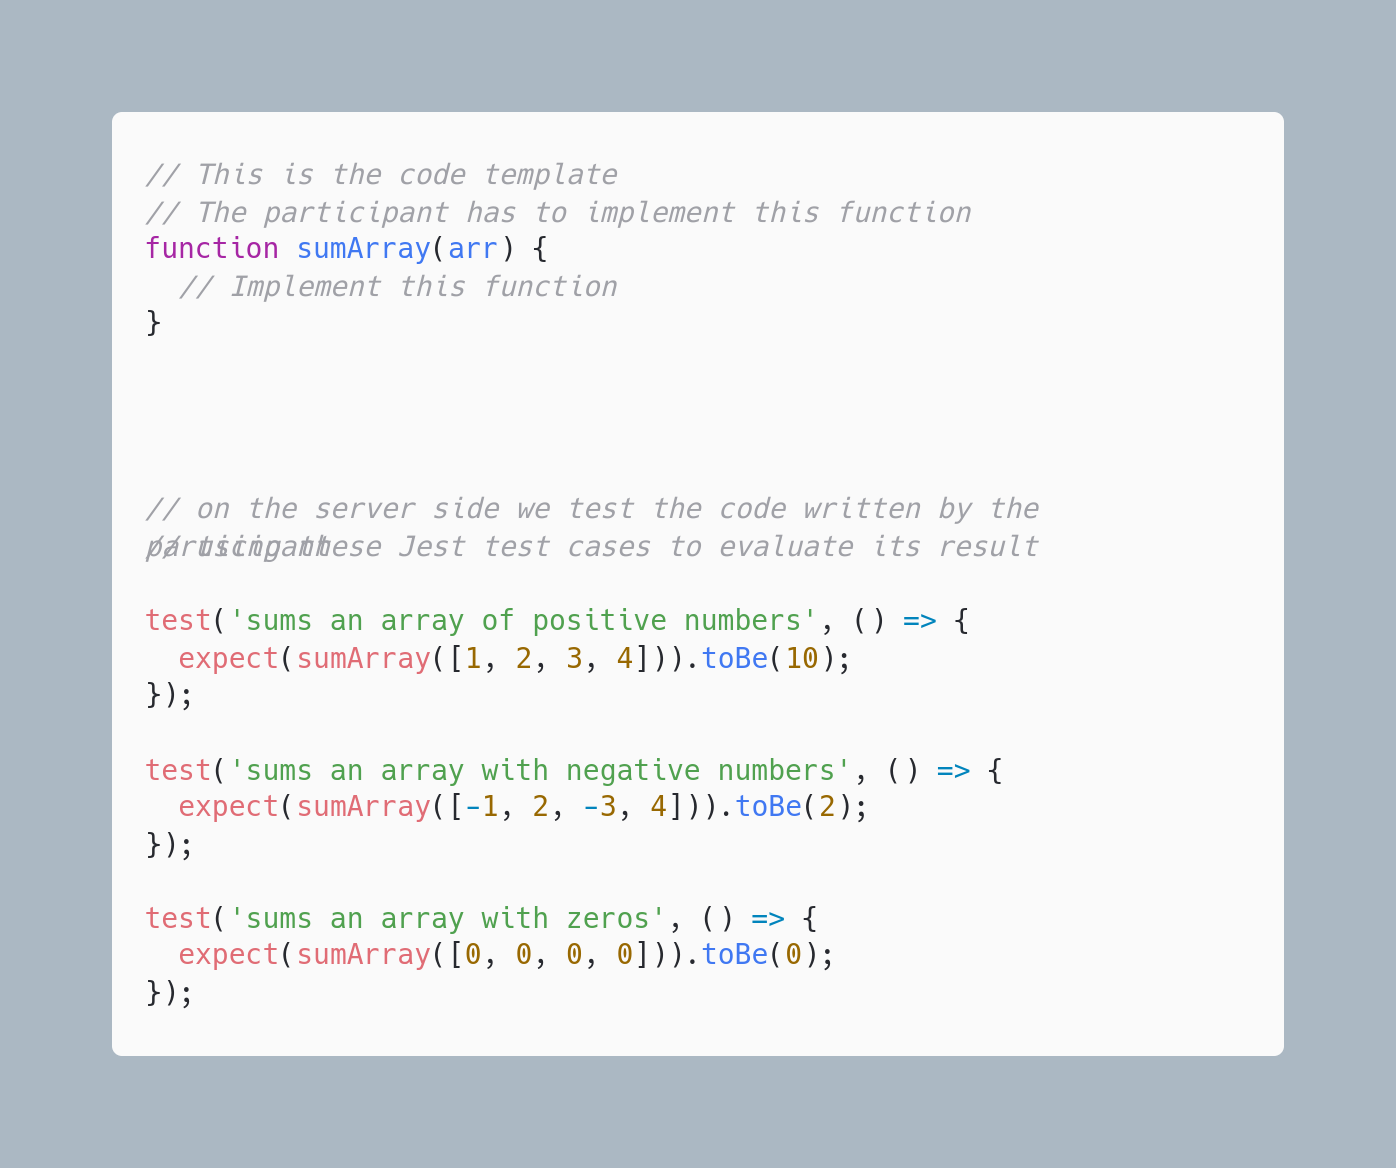
\includegraphics[width=0.9\textwidth]{images/approach2.png}
  \caption{Coding Problem With Unit Testing}\label{fig:approach2}
\end{figure}

For an instance, this approach is good because it looks clean and straight forward, but it has two drawbacks:
\begin{itemize}
  \item We need to setup up a testing environment for each problem, as an example we need to install Jest for javascript problems, JUnit for Java problems, etc.
  \item The output result of the execution will be hard to parse and can differ from one language to another.
\end{itemize}

\subsubsection{Approach 2: Using Argv and Stdout}
For this approach the goal was to pass the problem input arguments using Argv and get the output using Stdout.
then we can compare the output with the expected output to evaluate the result.

This approach is good because it is language agnostic, but it has some drawbacks:
\begin{itemize}
  \item It is really hard to deal with complex input data structures like arrays, objects, etc.
  \item for each problem code template we need to add the code to parse the input arguments and print the output.
\end{itemize}

the figure below \ref{fig:approach1} shows an example of a coding problem with test cases written in javascript:

\begin{figure}[h!]
  \centering
  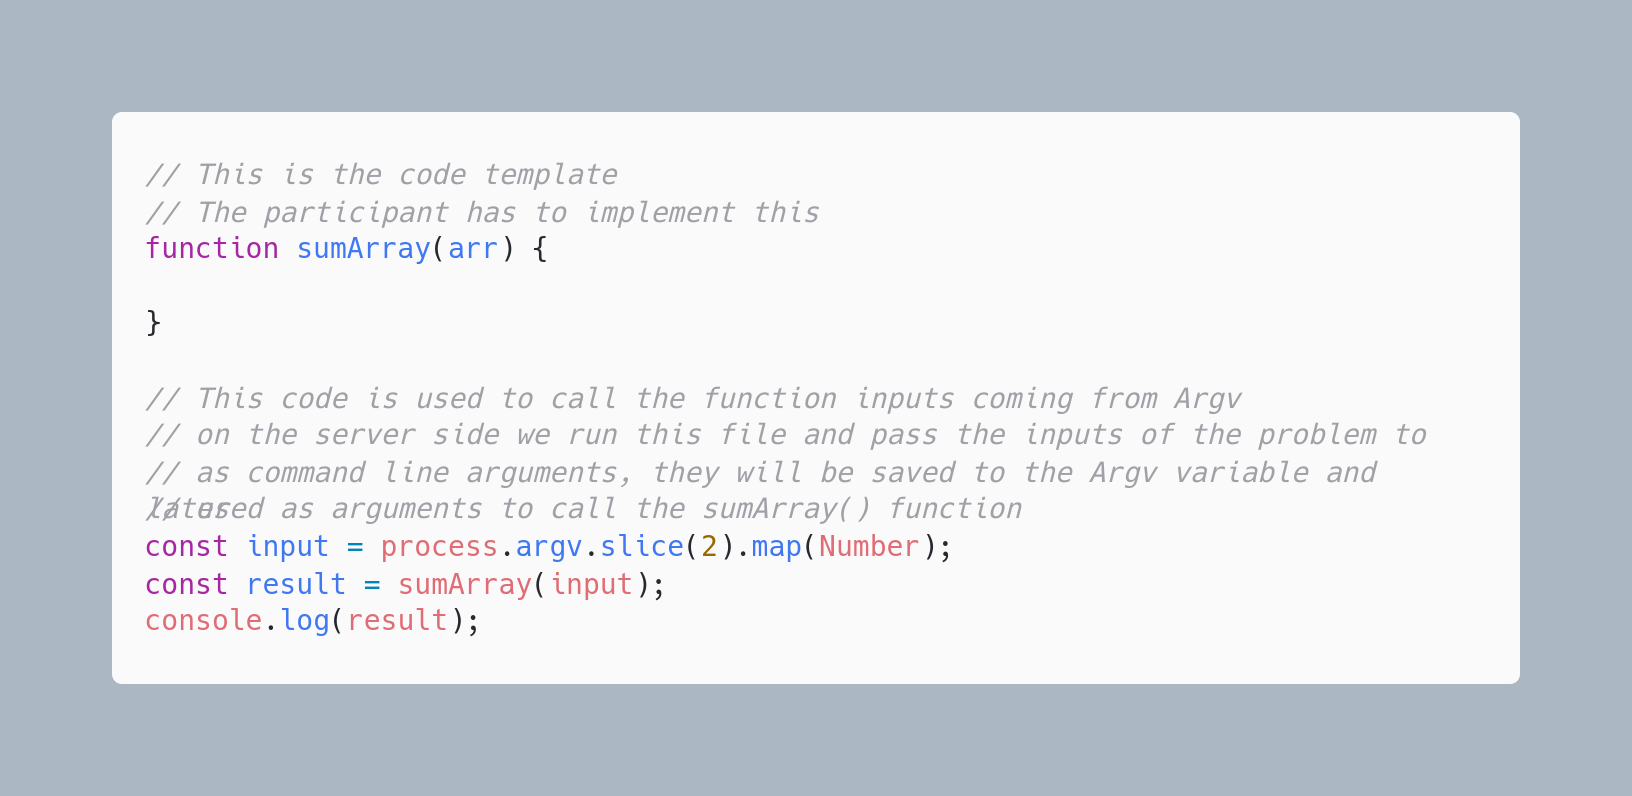
\includegraphics[width=0.9\textwidth]{images/approach1.png}
  \caption{Coding Problem With Argv and Stdout}\label{fig:approach1}
\end{figure}

\subsubsection{Approach 2: Merging Code With Written Test Cases}
In this approach we thought about writing the test cases for the coding problem,
these test cases will evaluate the code and return the result in a json format to the standard output.

The only drawback of this approach was:
\begin{itemize}
  \item We need to rewrite the test cases for each problem in each language that we want to support.
\end{itemize}

The figure below \ref{fig:approach3} shows an example of a coding problem with test cases written in javascript:

\begin{figure}[h!]
  \centering
  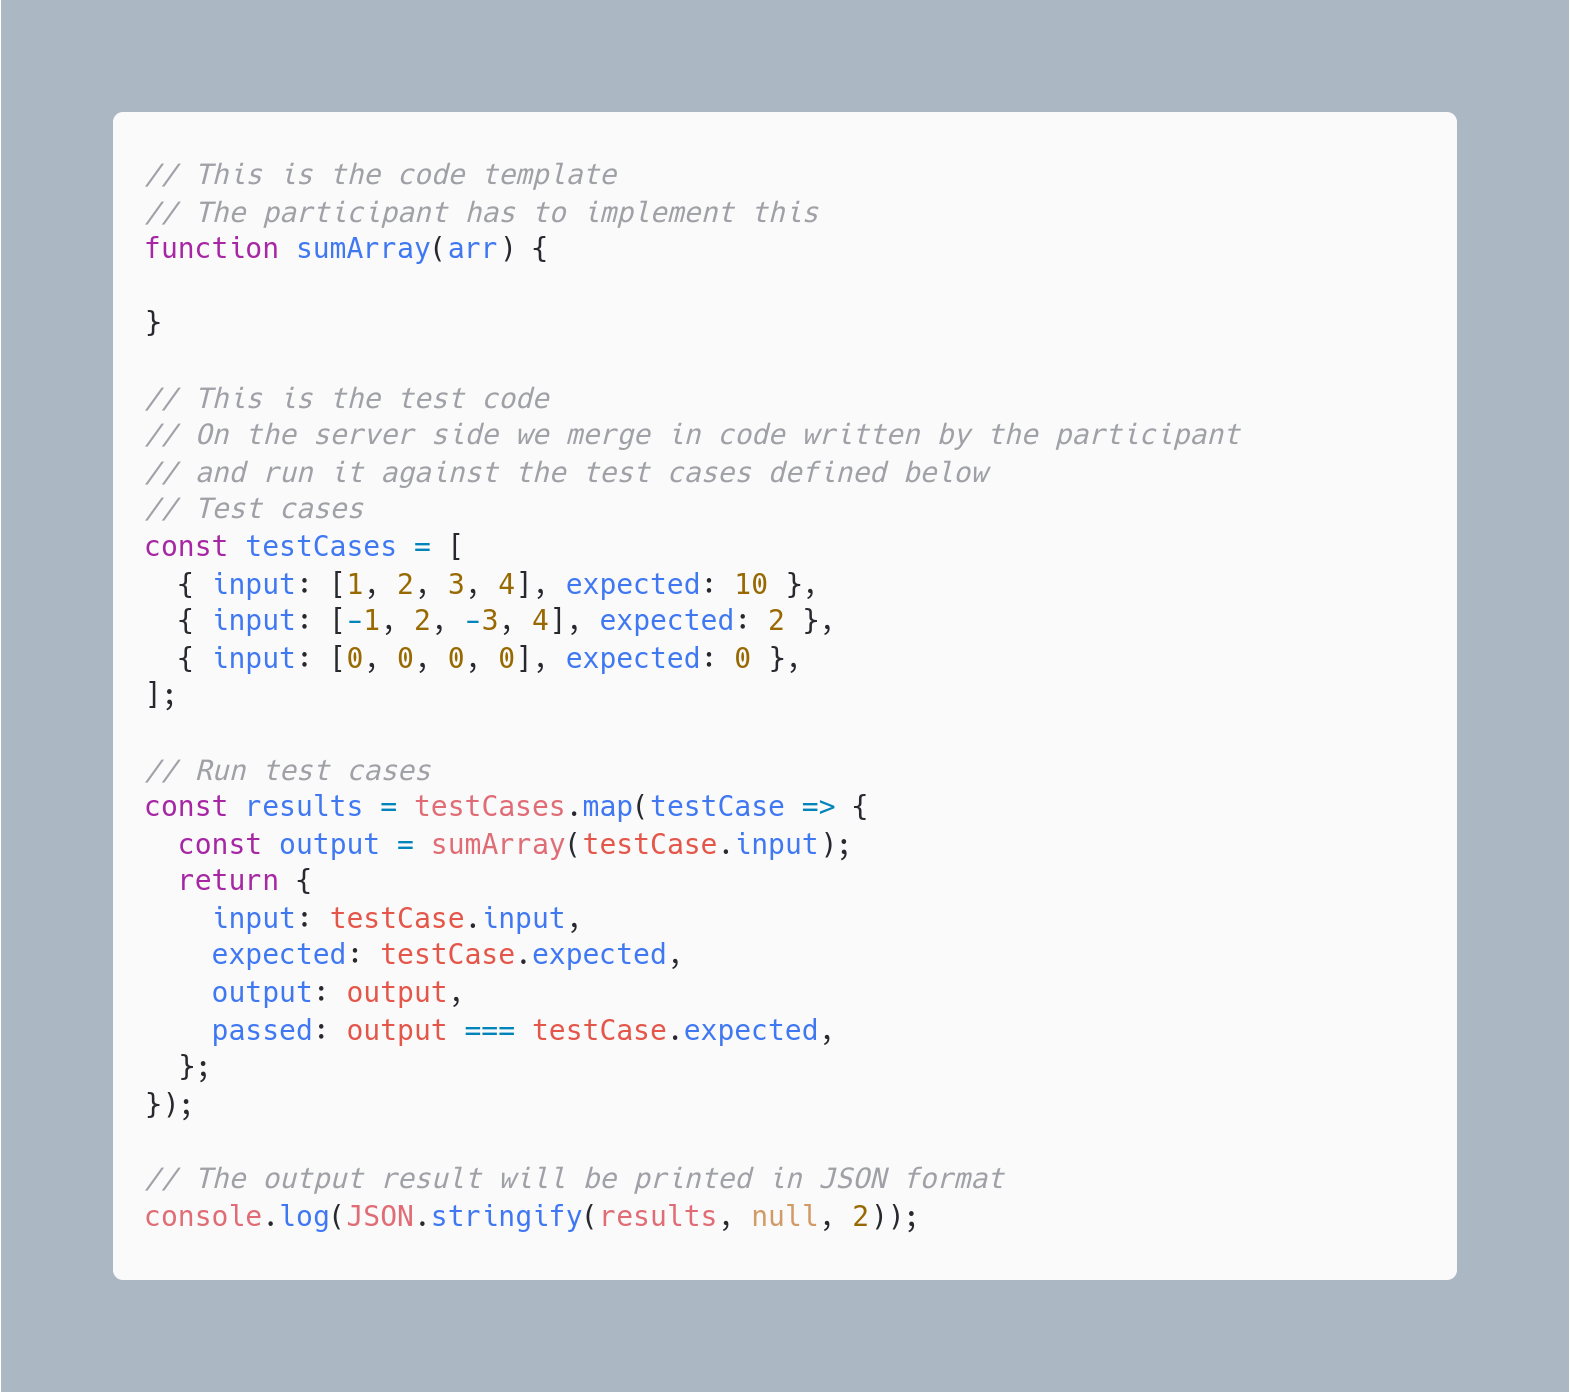
\includegraphics[width=0.9\textwidth]{images/approach3.png}
  \caption{Merging Code With Written Test Cases}\label{fig:approach3}
\end{figure}

\newpage
\subsection{Conclusion}
After comparing the tradeoffs of each approach, we decided to go with the third approach because it is the
most efficient and easy to implement and maintain.

Choosing this approach added only one constraint when creating a coding problem, the output of the test cases
should be always in the following format as shown in the figure below \ref{fig:output_format}:

\begin{figure}[h!]
  \centering
  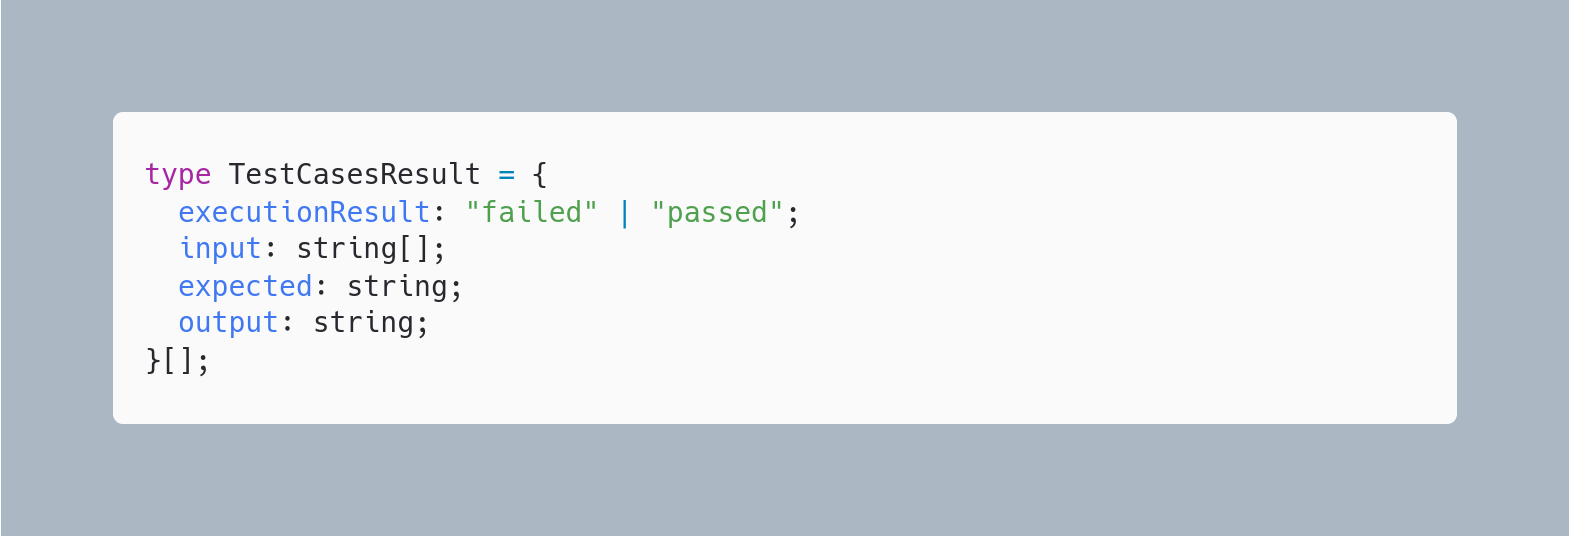
\includegraphics[width=0.9\textwidth]{images/testCasesResult.png}
  \caption{Test Cases Output Format}\label{fig:output_format}
\end{figure}

\newpage
\subsection{MongoDB Schema Diagram}
Since we are going to implement the coding problems, quizzes and tests management modules, we need to design
the database schema for each module. The figure below \ref{fig:db_schema} shows the database schema for the coding problems,
quizzes and tests management modules:

\begin{figure}[h!]
  \centering
  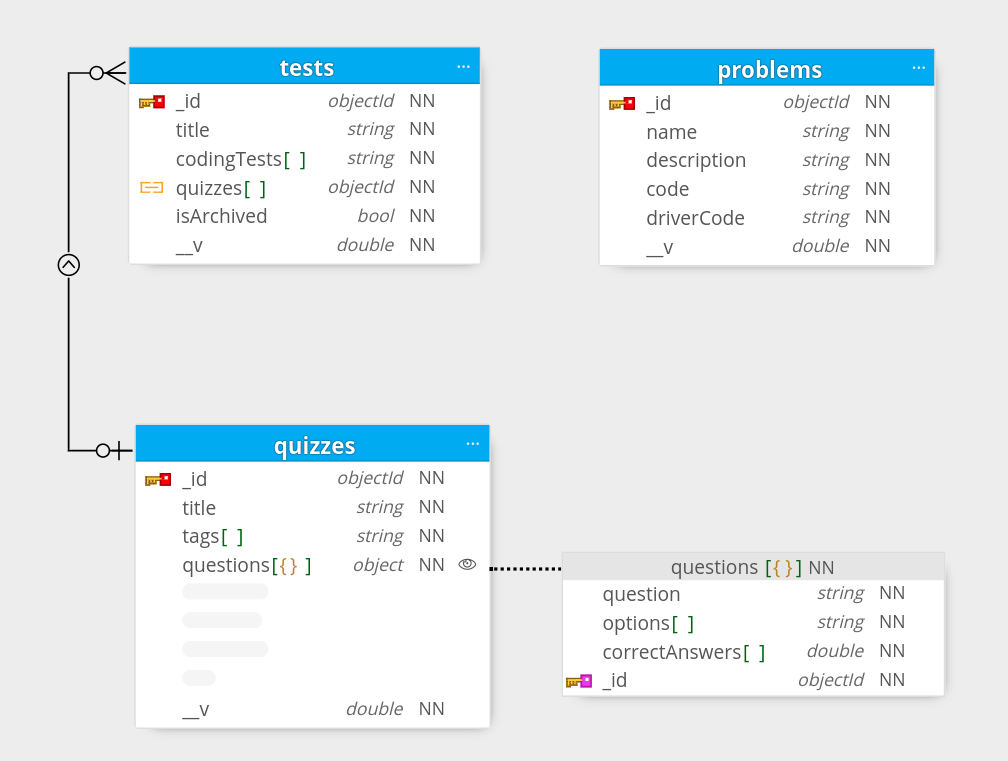
\includegraphics[width=0.9\textwidth]{images/sprint3Schema.png}
  \caption{Database Schema Diagram}\label{fig:db_schema}
\end{figure}

\subsection{API Endpoints}
One of the requirements for building the backend was to put the coding problems management into
its own API, as we might need to use it in other projects in the future. We decided to create a new
API called \textquotesingle{Coding Problems API}.

The rest of the APIs will be implemented in the main API codebase as we previously implemented the user management
module.

\subsubsection{Tests Management APIs}
In the test management module we added the following endpoints described in the table below \ref{table:testEndpoints}:

\begin{longtable}{|>{\centering\arraybackslash}p{6cm}|>{\centering\arraybackslash}p{8cm}|}
  \hline
  \rowcolor{blue!20} \textbf{Endpoint} & \textbf{Description}    \\ \hline
  \texttt{GET /api/test/}              & Fetch all tests         \\ \hline
  \texttt{POST /api/test/create}       & Create a new test       \\ \hline
  \texttt{PUT /api/test/update}        & Update an existing test \\ \hline
  \texttt{DELETE /api/test/delete/:id} & Delete a test by ID     \\ \hline
  \texttt{POST /api/test/search}       & Search for tests        \\ \hline
  \caption{API Endpoints for Test Management} \label{table:testEndpoints}
\end{longtable}

\subsubsection{Quizzes Management APIs}
The quizzes management module will have the following endpoints described in the table below \ref{table:quizEndpoints}:

\begin{longtable}{|>{\centering\arraybackslash}p{6cm}|>{\centering\arraybackslash}p{8cm}|}
  \hline
  \rowcolor{blue!20} \textbf{Endpoint} & \textbf{Description}    \\ \hline
  \texttt{GET /api/quiz/}              & Fetch all quizzes       \\ \hline
  \texttt{POST /api/quiz/create}       & Create a new quiz       \\ \hline
  \texttt{PUT /api/quiz/update}        & Update an existing quiz \\ \hline
  \texttt{DELETE /api/quiz/delete/:id} & Delete a quiz by ID     \\ \hline
  \texttt{POST /api/quiz/search}       & Search for quizzes      \\ \hline
  \caption{API Endpoints for Quiz Management} \label{table:quizEndpoints}
\end{longtable}

\subsubsection{Coding Problems Management APIs}
The coding problems management module will have the following endpoints described in the table below \ref{table:problemEndpoints}:

\begin{longtable}{|>{\centering\arraybackslash}p{6cm}|>{\centering\arraybackslash}p{8cm}|}
  \hline
  \rowcolor{blue!20} \textbf{Endpoint}          & \textbf{Description}              \\ \hline
  \texttt{GET /api/problem/get-problem/:id}     & Fetch a coding problem by ID      \\ \hline
  \texttt{POST /api/problem/create-problem}     & Create a new coding problem       \\ \hline
  \texttt{GET /api/problem/get-problems}        & Fetch all coding problems         \\ \hline
  \texttt{POST /api/problem/execute}            & Execute code for a coding problem \\ \hline
  \texttt{POST /api/problem/test-problem}       & Test a coding problem             \\ \hline
  \texttt{PUT /api/problem/update-problem/:id}  & Update a coding problem by ID     \\ \hline
  \texttt{POST /api/problem/search-problem}     & Search for coding problems        \\ \hline
  \texttt{POST /api/problem/search-problems}    & Search for coding problems by IDs \\ \hline
  \texttt{GET /api/problem/get-problems-by-ids} & Fetch coding problems by IDs      \\ \hline
  \caption{API Endpoints for Coding Problem Management} \label{table:problemEndpoints}
\end{longtable}

\subsubsection{Piston API Endpoints}
The Piston API will have the following endpoints described in the table below \ref{table:pistonEndpoints}:

\begin{longtable}{|>{\centering\arraybackslash}p{6cm}|>{\centering\arraybackslash}p{8cm}|}
  \hline
  \rowcolor{blue!20} \textbf{Endpoint} & \textbf{Description}           \\ \hline
  \texttt{GET /runtimes}               & Get supported runtimes         \\ \hline
  \texttt{POST /execute}               & execute code                   \\ \hline
  \texttt{POST /versions}              & get available runtime versions \\ \hline
  \caption{Piston API Endpoints} \label{table:pistonEndpoints}
\end{longtable}

\section{Impelementation}
After finishing the analysis and design phase, we started implementing the coding problems, quizzes and tests management modules.
we ended up with Two APIs, the main API and the coding problems API Along with the Piston API to execute the code.
the table below shows each API and its port number:

\begin{longtable}{|>{\centering\arraybackslash}p{6cm}|>{\centering\arraybackslash}p{8cm}|}
  \hline
  \rowcolor{blue!20} \textbf{Endpoint} & \textbf{Description} \\ \hline
  \texttt{Coding Problems API}         & 2000                 \\ \hline
  \texttt{Main API}                    & 5000                 \\ \hline
  \texttt{Piston}                      & 5001                 \\ \hline
  \caption{Service Ports}\label{tab:service_ports}
\end{longtable}

The figure below \ref{fig:services} displays all the three APIs up and running:

\begin{sidewaysfigure}[h!]
  \centering
  \setlength\fboxsep{0pt} % Adjusts the separation between the image and the border
  \setlength\fboxrule{2pt} % Adjusts the thickness of the border
  \fcolorbox{orange}{white}{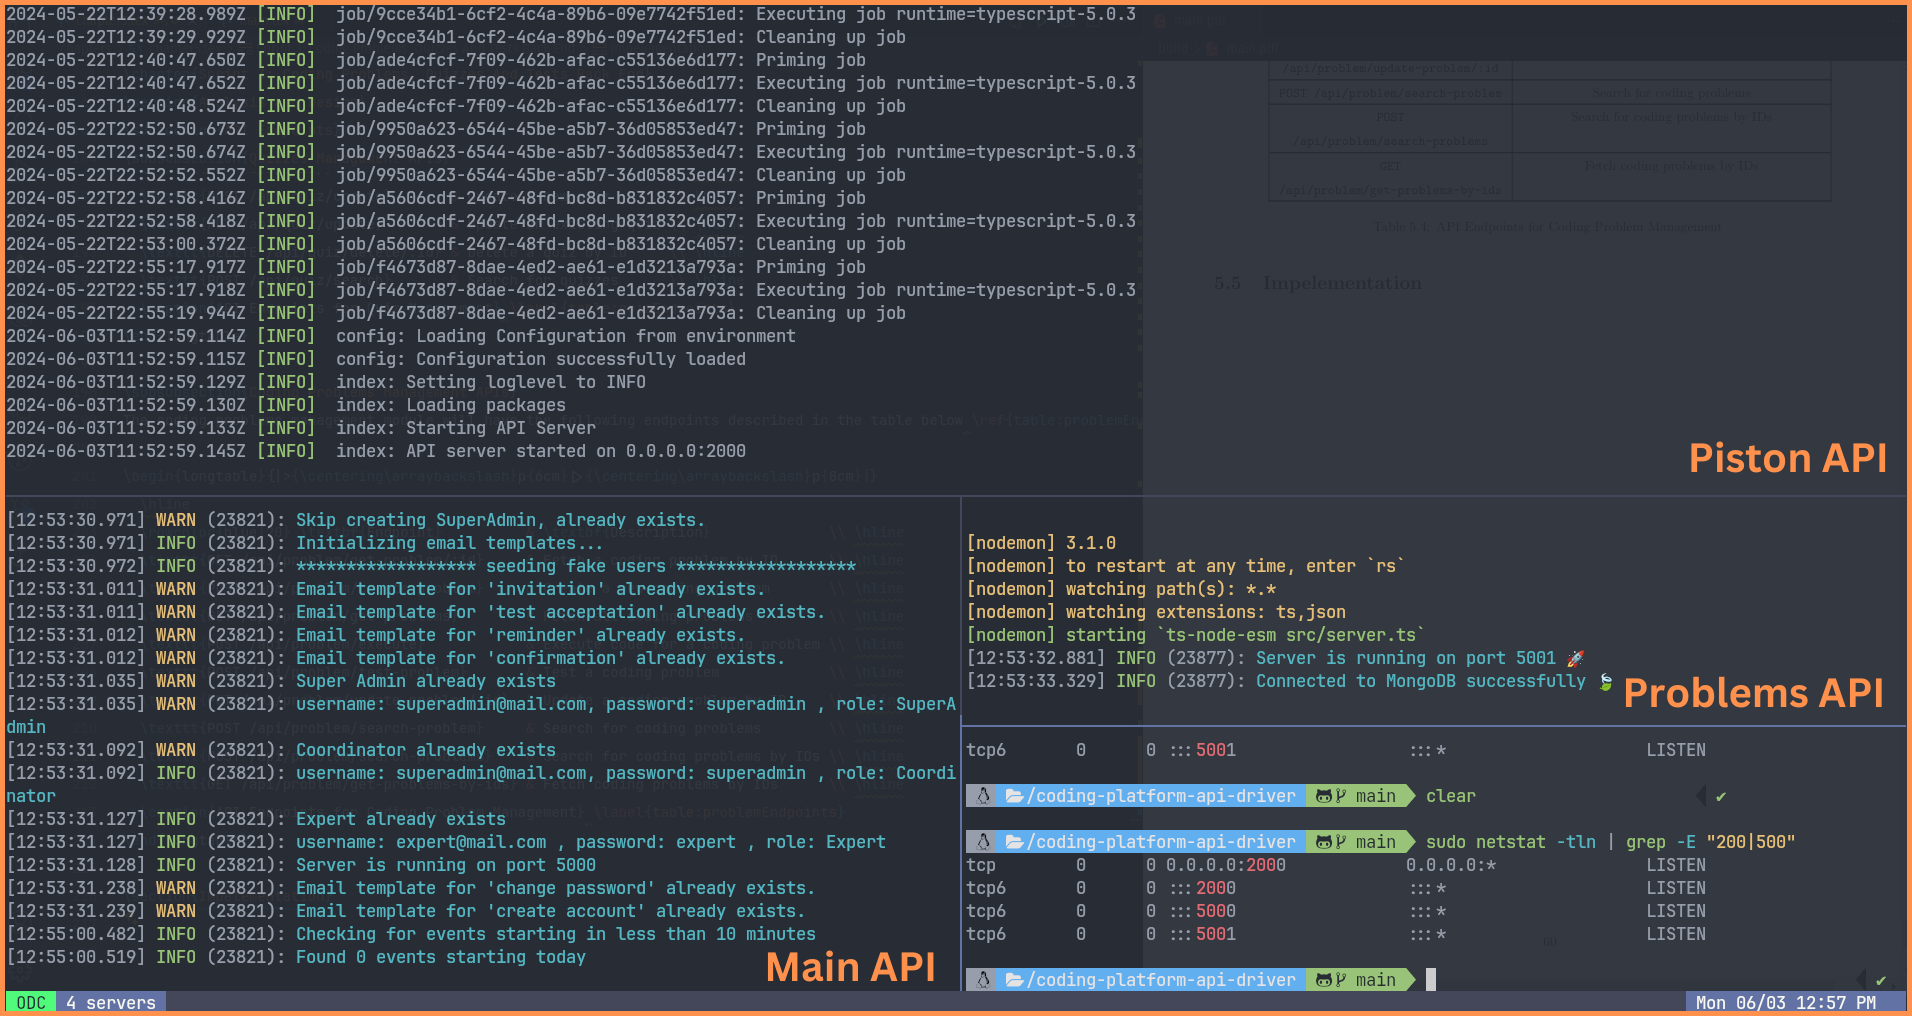
\includegraphics[width=0.8\paperheight, height=0.75\paperwidth]{images/services.png}}
  \caption{All Services Running}\label{fig:services}
\end{sidewaysfigure}




